% =====================================================================
%  ECONSCHOOL — PROBLEMS SHEET
%  One solved problem (with a TikZ figure) + one near-twin exercise.
%
%  Compile:  pdflatex perfect-substitutes.tex   (run twice for the footer)
%  No font installation needed: text and maths are Computer Modern
%  (Latin Modern where available), the same maths face the site renders
%  with KaTeX.
% =====================================================================
\documentclass[11pt]{article}

% ---- Fonts ----------------------------------------------------------
% Latin Modern if available (it is on MacTeX); base Computer Modern
% otherwise. Either way the maths face is Computer Modern.
\IfFileExists{lmodern.sty}{\usepackage[T1]{fontenc}\usepackage{lmodern}}{}

% ---- Core packages --------------------------------------------------
\usepackage{amsmath,amssymb}
\usepackage[a4paper,top=2.3cm,bottom=2.4cm,left=2.6cm,right=2.6cm]{geometry}
\usepackage{graphicx}
\usepackage{xcolor}
\usepackage{microtype}
\usepackage{enumitem}

% ---- Figures --------------------------------------------------------
\usepackage{tikz}
\usepackage{pgfplots}
\pgfplotsset{compat=1.18}
\usetikzlibrary{arrows.meta}

% ---- Layout ---------------------------------------------------------
\setlist[enumerate]{leftmargin=1.6em,itemsep=0.35em,topsep=0.3em}
\setlist[itemize]{leftmargin=1.6em,itemsep=0.2em,topsep=0.2em}
\setlength{\parindent}{0pt}
\setlength{\parskip}{0.6em}
\linespread{1.05}

% ---- Brand palette (mirrors src/styles/global.css) ------------------
\definecolor{bg}{HTML}{FAF7F2}             % cream background
\definecolor{ink}{HTML}{2A2620}            % body text
\definecolor{inksoft}{HTML}{4A4239}        % secondary text
\definecolor{inkfaint}{HTML}{7A6F62}       % tertiary / italics
\definecolor{violet}{HTML}{5A1BA6}         % titles, indifference curves
\definecolor{violetsoft}{HTML}{7A4FC4}     % sub-headings
\definecolor{terracotta}{HTML}{A03A2C}     % accents, links, budget line
\definecolor{terracottasoft}{HTML}{C66B5B} % light fills
\definecolor{sage}{HTML}{8AA08A}           % dividers
\definecolor{sagesoft}{HTML}{C8D2C0}       % footer rule
\definecolor{rule}{HTML}{E5DDD0}           % hairline rules

% ---- Figure styles --------------------------------------------------
% A small reusable set for the diagrams these sheets need. Add curve
% colours per topic (demand/supply, cost curves, ...) as required.
\pgfplotsset{
  microecon/.style={
    width=8.4cm, height=6.4cm,
    axis lines=middle,
    axis line style={-{Stealth[length=2mm]}, ink},
    tick label style={font=\footnotesize, color=inksoft},
    label style={font=\small, color=inksoft},
    every axis x label/.style={at={(ticklabel* cs:1.02)}, anchor=west},
    every axis y label/.style={at={(ticklabel* cs:1.02)}, anchor=south},
    xmin=0, ymin=0,
    tick align=outside,
    enlargelimits=false,
  },
}
\tikzset{
  indiff/.style={ink, thick},                     % indifference curve
  budget/.style={terracotta, thick},                 % budget line
  optimum/.style={circle, fill=violet, inner sep=1.6pt},  % optimal bundle
}

% ---- Document colour ------------------------------------------------
\color{ink}
\pagecolor{bg}        % cream page; comment out this line for white

% ---- Links ----------------------------------------------------------
\usepackage[hidelinks]{hyperref}
\hypersetup{colorlinks=true, urlcolor=terracotta, linkcolor=terracotta}

% ---- Small reusable pieces ------------------------------------------
\newcommand{\eyebrow}[1]{{\color{terracotta}\textls[110]{\scshape #1}}}
% ES mark: the logo if present, a typographic fallback otherwise.
\newcommand{\esmark}{%
  \IfFileExists{es-logo.png}
    {\raisebox{-0.34\height}{
\includegraphics[height=5mm]{es-logo.png}}}
    {{\color{violet}\fontsize{20}{20}\selectfont\scshape ES}}}
\newcommand{\sagerule}{\par\vspace{0.25em}{\color{sage}\rule{\linewidth}{0.6pt}}\par\vspace{0.15em}}
\newcommand{\heading}[1]{\par\vspace{1.1em}{\color{violet}\large\bfseries #1}\par\vspace{0.25em}}
\newcommand{\subheading}[1]{\par\vspace{0.7em}{\color{violetsoft}\bfseries #1}\par\vspace{0.1em}}
\newcommand{\MU}{\mathrm{MU}}   % upright marginal-utility symbol

% ---- Footer ---------------------------------------------------------
\usepackage{fancyhdr}
\pagestyle{fancy}
\fancyhf{}
\renewcommand{\headrulewidth}{0pt}
\renewcommand{\footrulewidth}{0.4pt}
\renewcommand{\footrule}{{\color{sagesoft}%
  \vskip-\footruleskip\vskip-\footrulewidth
  \hrule height\footrulewidth width\headwidth}}
\fancyfoot[L]{\color{inkfaint}\footnotesize econschool.in}
\fancyfoot[C]{\color{inkfaint}\footnotesize\thepage}
\fancyfoot[R]{\color{inkfaint}\footnotesize youtube.com/@econ.school}

% =====================================================================
\begin{document}

% ---------- Masthead -------------------------------------------------
\noindent
\begin{tabular*}{\linewidth}{@{}l@{\extracolsep{\fill}}r@{}}
  \eyebrow{To go with the lectures} & \esmark
\end{tabular*}
\sagerule

% ---------- Title (replace per sheet) --------------------------------
{\color{violet}\fontsize{26}{30}\selectfont Perfect substitutes\par}
\vspace{0.2em}
{\color{inkfaint}\itshape Consumer theory \;\textperiodcentered\; Problem~1
 \quad\textperiodcentered\quad
 Video: \href{https://youtu.be/qKRKmEKNqFQ}{youtu.be/qKRKmEKNqFQ}\par}
\sagerule

% =====================================================================
\heading{Solved problem}

A student has a weekly food budget of $M=\$20$ to spend on two goods:
\begin{itemize}
  \item $x$: packets of instant noodles, at $p_x=\$4$ each;
  \item $y$: cups of fruit yogurt, at $p_y=\$5$ each.
\end{itemize}

Preferences are represented by $u(x,y)=x+2y$, so one more cup of yogurt is worth twice as much as one more packet of noodles. Find the optimal bundle $(x^\star,y^\star)$ and illustrate the budget line and the optimal choice in a diagram.

\subheading{Solution}
Here we solve the following problem:
\begin{eqnarray*} \max_{(x,y)\in \mathbb{R}^2_+} & x + 2y \\ \text{s.t.} & 4x + 5y \leq 20 \end{eqnarray*}

Compare the marginal utility per dollar spent on each good:
\[
  \frac{\MU_x}{p_x}=\frac{1}{4}
  \qquad\text{and}\qquad
  \frac{\MU_y}{p_y}=\frac{2}{5}.
\]
Since $\MU_x/p_x < \MU_y/p_y$, every dollar buys more utility on yogurt, so the student spends the whole budget on $y$. With $M=20$ and $p_y=5$, the optimal bundle is
\[
  (x^\star,y^\star)=\Bigl(0,\tfrac{M}{p_y}\Bigr)=(0,4).
\]

\begin{center}
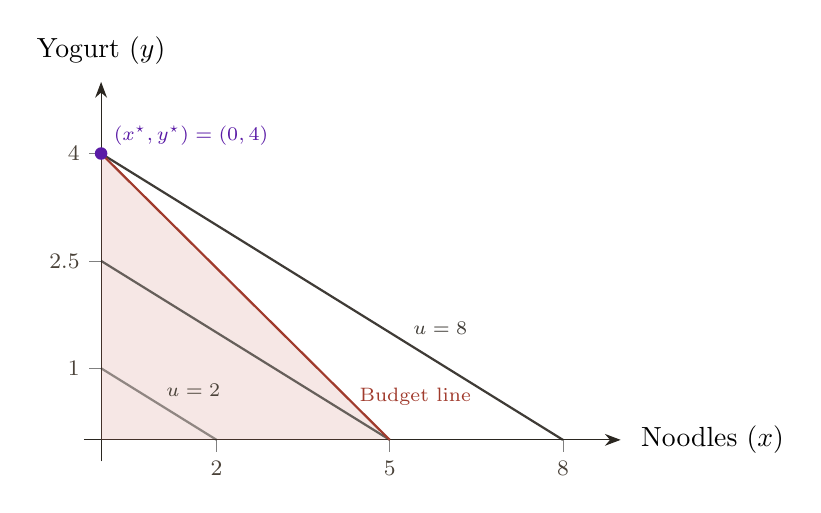
\begin{tikzpicture}
  \begin{axis}[
      microecon,
      xmin=-0.3, xmax=9, ymin=-0.3, ymax=5,
      xlabel={Noodles ($x$)}, ylabel={Yogurt ($y$)},
      xtick={2,5,8}, ytick={1,2.5,4},
      clip mode=individual,
  ]
    % Budget set: the affordable triangle (0,0)-(5,0)-(0,4)
    \addplot[draw=none, fill=terracottasoft, fill opacity=0.16]
      coordinates {(0,0) (5,0) (0,4)} \closedcycle;

    % Indifference curves: u = x + 2y  =>  y = u/2 - x/2  (slope -1/2).
    % Two levels are labelled to show utility rising up and to the right;
    % the middle curve is left unlabelled as visual context.
    \addplot[indiff, opacity = 0.5, domain=0:2] {1   - 0.5*x}
      node[pos=0.5, above right=-1pt, font=\scriptsize, text=inksoft, opacity=1] {$u=2$};
    \addplot[indiff, opacity = 0.7, domain=0:5] {2.5 - 0.5*x};
    \addplot[indiff, opacity = 0.9, domain=0:8] {4 - 0.5*x}
      node[pos=0.66, above right=-1pt, font=\scriptsize, text=ink] {$u=8$};

    % Budget line: 4x + 5y = 20  =>  y = 4 - 0.8x  (slope -4/5)
    \addplot[budget, domain=0:5] {4 - 0.8*x}
      node[pos=0.85, right=1pt, font=\scriptsize, text=terracotta] {Budget line};

    % Optimum at the corner (0,4)
    \node[optimum] at (axis cs:0,4) {};
    \node[font=\scriptsize, anchor=west, text=violet]
      at (axis cs:0.05,4.25) {$(x^\star,y^\star)=(0,4)$};
  \end{axis}
\end{tikzpicture}
\end{center}
\vspace{-0.2em}
{\color{inkfaint}\footnotesize\itshape
 Figure~1.\enspace Indifference curves are straight lines $x+2y=\bar u$ with
 absolute slope $\MU_x/\MU_y=1/2$. The budget line has absolute slope
 $p_x/p_y=4/5$ and is steeper, so the highest attainable indifference curve is
 reached at the corner $(0,4)$, where the budget line meets the $y$-axis.\par}
\sagerule

% =====================================================================
\heading{Exercise}

A student commutes to university by either:
\begin{itemize}
  \item $x$: bus rides;
  \item $y$: metro rides.
\end{itemize}

Each ride, by either mode, is one trip to university, so the student treats the two modes as perfect substitutes:
\[
  u(x,y)=x+y.
\]
A bus ride costs $p_x=\$20$ and a metro ride $p_y=\$30$, and the weekly transport budget is $M=\$180$.

\begin{enumerate}
  \item Draw the budget set and the budget line.

  \item Compute the marginal utility per dollar spent on each mode, $\dfrac{\MU_x}{p_x}$ and $\dfrac{\MU_y}{p_y}$. Find the utility-maximising bundle $(x^\star,y^\star)$.

  \item Suppose the metro authority introduces a discounted student fare, cutting the metro price to $p_y=\$20$. With everything else unchanged, characterise the set of utility-maximising bundles.
\end{enumerate}

\subheading{Extension: quality-adjusted travel}

Suppose instead the student finds the metro more convenient, because it is faster and more reliable, so preferences become
\[
  u(x,y)=x+1.5\,y,
\]
with the original prices and budget, $p_x=\$20$, $p_y=\$30$, and $M=\$180$.

\begin{enumerate}
  \setcounter{enumi}{3}
  \item Solve for the utility-maximising bundle(s) under these preferences.
\end{enumerate}

\medskip
{\color{inksoft}\emph{Checking your work.}\enspace To discuss the exercise, join
 the community forum at \href{https://econschool.in}{econschool.in}.\par}

\end{document}
